%==========================================================================
% IEEE-format report (conference/IEEEtran two-column).
% Compile on Overleaf: New Project -> Upload -> add this file, references.bib,
% and the results/*.png figures (see report/README.md for the figure list).
% Engine: pdfLaTeX; run twice + BibTeX (Overleaf does this automatically).
%==========================================================================
\documentclass[conference]{IEEEtran}
\IEEEoverridecommandlockouts

\usepackage{cite}
\usepackage{amsmath,amssymb}
\usepackage{graphicx}
\usepackage{booktabs}
\usepackage{url}
\usepackage{xcolor}
\usepackage[hidelinks]{hyperref}

% Figures are the PNGs from ../results/. On Overleaf, upload them into a
% folder named "figures" (or edit this path to match your upload).
\graphicspath{{figures/}{../results/}}

\begin{document}

\title{A Real-Measurement Reappraisal of Post-Quantum Cryptography for
Constrained IoT: Benchmarks, Hybrid Key Exchange, Timing Analysis, and
Device-Class Guidance}

\author{\IEEEauthorblockN{Rakshit}
\IEEEauthorblockA{Cryptography and Network Security --- Course Project\\
Extending Narayanan \textit{et al.} (2026), DOI: 10.1007/s40998-025-01002-1}}

\maketitle

\begin{abstract}
Post-quantum cryptography (PQC) is now standardised (NIST FIPS 203/204/205),
and recent frameworks such as PQShield-IoT (Narayanan \textit{et al.}, 2026)
integrate it with permissioned blockchains for secure IoT edge communication.
That framework, however, is evaluated \emph{entirely in simulation}
(Contiki-NG/NS-3) and reports per-operation latencies with no stated measurement
methodology, fixes on a single signature scheme (Dilithium2), employs
\emph{pure} rather than hybrid PQC, and reports no side-channel analysis.
We address these gaps on commodity hardware. We (i) benchmark classical
versus post-quantum key-encapsulation and signature primitives from real
implementations (PQClean via \texttt{pqcrypto}; OpenSSL via \texttt{cryptography}),
reporting time and bytes-on-wire for sixteen schemes; (ii) build a socket-based
classical/post-quantum/\emph{hybrid} key-exchange prototype and measure the cost
of hybrid ``insurance''; (iii) demonstrate a timing side-channel and test
ML-KEM decapsulation for a timing oracle; and (iv) extrapolate to the ARM
Cortex-M4 using the public pqm4 dataset and derive an RFC 7228 device-class
recommendation matrix. Two headline findings: on CPU-class hardware,
standardised lattice PQC costs microseconds---its real price is bytes on the
wire (768--2420\,B versus 32--65\,B), not computation; and the base paper's four
reported cryptographic latencies imply four different processor clocks spanning
25--189\,MHz when divided into measured Cortex-M4 cycle counts, so they cannot be
cycle-accurate measurements of the device it declares---a clock-independent
demonstration of the risk of reporting timings without a methodology.
Hybrid X25519+ML-KEM-768 adds only 64\,B and sub-millisecond overhead over pure
ML-KEM, making defence-in-depth nearly free.
\end{abstract}

\begin{IEEEkeywords}
Post-quantum cryptography, ML-KEM, ML-DSA, Falcon, SPHINCS+, hybrid key
exchange, IoT, side-channel, benchmarking, RFC 7228.
\end{IEEEkeywords}

\section{Introduction}
Shor's algorithm renders RSA and elliptic-curve cryptography insecure against
a sufficiently large quantum computer, retro-actively threatening any data
recorded today (``harvest-now, decrypt-later''). NIST concluded its main PQC
standardisation in 2024 with ML-KEM (FIPS 203)~\cite{fips203}, ML-DSA (FIPS
204)~\cite{fips204}, and SLH-DSA (FIPS 205)~\cite{fips205}. Deploying these on
resource-constrained IoT edge devices is the open engineering problem.

PQShield-IoT~\cite{narayanan2026pqshield} is a representative recent framework:
it combines Kyber512 (KEM) and Dilithium2 (signatures) with AES-256-GCM, a
SHA3-256 key-derivation function, and a permissioned blockchain for identity
and access management. It is a well-integrated design, but its evaluation is
\emph{simulated} on ARM Cortex-M4F profiles in Contiki-NG/NS-3. It states that
PQClean and liboqs supplied the cryptographic code, yet reports per-operation
latencies without specifying the execution host, the timing method, the
repetition count, or any variance---so those figures cannot be attributed to a
measurement. From a careful reading we identify four gaps and address them with
laptop-only, reproducible experiments:

\begin{enumerate}
\item \textbf{Pure PQC, no hybrid.} Real migrations (TLS~1.3
  X25519MLKEM768~\cite{x25519mlkem768}) combine classical and post-quantum
  key exchange so a single cryptanalytic advance does not collapse security.
\item \textbf{Timings without a methodology.} The reported latencies specify no
  host, no timing procedure, no repetition count and no variance, and the device
  is an emulated profile rather than silicon---so they are unverifiable.
\item \textbf{Single signature scheme.} Dilithium2 only; no comparison with
  Falcon or SPHINCS+, whose size/speed profiles differ by orders of magnitude.
\item \textbf{No timing/side-channel analysis.}
\end{enumerate}

\noindent Our contributions map one-to-one onto these gaps, plus a fifth
integrative artefact: a Cortex-M4 extrapolation and an RFC 7228~\cite{rfc7228}
device-class recommendation matrix.

\section{Background and Related Work}
\textbf{Standardisation.} ML-KEM and ML-DSA are lattice schemes (Module-LWE);
SLH-DSA is hash-based (conservative security); Falcon (FN-DSA, FIPS 206 draft)
offers compact lattice signatures via NTRU trapdoor sampling. In 2025 NIST
selected the code-based KEM HQC as a backup to ML-KEM, hedging against a
lattice-specific break. Grover's algorithm only halves symmetric security, so
AES-256-GCM and SHA3-256 remain adequate and are retained here.

\textbf{PQC on constrained hardware.} The community benchmark is
pqm4~\cite{kannwischer2019pqm4}, measuring NIST candidates on the Cortex-M4 in
cycles, code size, and stack. Testbed studies (Bozhko \textit{et
al.}~\cite{bozhko2023pqtls}; Hanna \textit{et al.}~\cite{hanna2025pqtls})
evaluate PQ-TLS on real IoT but not the framework-integration setting.

\textbf{Blockchain-integrated PQC for IoT.} PQShield-IoT extends a line
including STarEdgeChain~\cite{mollah2024staredgechain},
THASSA~\cite{khan2024thassa}, and lattice+blockchain authentication
schemes~\cite{sarkar2024lattice,kuang2025lightweight,prajapat2025quantumsafe,erukala2025hybrid,wang2024lattice}.
A recurring limitation across this thread---which the base paper does not fully
escape---is the absence of real constrained-hardware measurement.

\textbf{Side channels.} Constant-time implementation is essential: the
KyberSlash attacks~\cite{kyberslash2024} recovered Kyber keys from
secret-dependent division timing in decapsulation. ML-KEM's IND-CCA2 guarantee
depends on a constant-time Fujisaki--Okamoto implicit-rejection path.

\section{Methodology}
All experiments run on an Intel Core i5-13500H laptop, Windows~11, Python
3.14, with the process pinned to one performance core at high priority. PQC
uses \texttt{pqcrypto}~0.4.0 (PQClean~\cite{pqclean} portable C, no AVX2);
classical uses \texttt{cryptography}~49.0.0 (OpenSSL, optimised assembly). We
deliberately note this asymmetry: classical numbers use hand-tuned assembly
while PQC uses portable C, so every classical-versus-PQC gap is an
\emph{upper bound} on PQC cost.

\textbf{Benchmark suite.} We time keygen/encapsulate/decapsulate (KEM) and
keygen/sign/verify (signature) with a monotonic \texttt{perf\_counter\_ns}
clock, time-based warm-up, the garbage collector disabled inside the timed
region, and \emph{batched} sampling for sub-millisecond operations (each
sample is the mean of $k$ calls, $k$ sized so a sample spans $\geq$10\,ms) to
defeat timer granularity and scheduler quanta. The median is the headline
statistic (OS noise is one-sided). Signatures are over a 59-byte message (the
SUPERCOP/pqm4 convention). Calibration rows measure fixed per-call overhead.

\textbf{Hybrid handshake.} A length-prefixed TCP client/server performs a
one-round-trip key exchange in three modes---pure X25519, pure ML-KEM, and
hybrid---with the session key $K=\mathrm{SHA3\text{-}256}(\text{label}\,\|\,
\text{mode}\,\|\,\text{level}\,\|\,ss_{\mathrm{cls}}\,\|\,ss_{\mathrm{pq}}\,\|\,
\text{transcript})$ (concatenation combiner) followed by an AES-256-GCM
``finished'' exchange for key confirmation. Modelling SHA3-256 as a random
oracle, the key is indistinguishable from random while either shared secret is
unknown, and the transcript binds both ciphertexts, giving a robust
combiner~\cite{tls13hybrid}. We measure handshake latency and exact
bytes-on-wire.

\textbf{Timing analysis.} (A) We measure MAC-tag rejection time versus
matching-prefix length for a naive early-exit comparison, C \texttt{memcmp},
and \texttt{hmac.compare\_digest}. (B) We test ML-KEM-512 decapsulation over
valid, one-bit-flipped, and random ciphertexts for a timing oracle. Classes
are \emph{interleaved} (round-robin) so thermal drift cannot masquerade as a
class difference, and inputs are drawn from pools; verdicts use the monotonic
trend (Pearson $r$) with a Welch $z$-gate, not $z$ alone.

\textbf{Extrapolation.} We combine our desktop medians with pqm4's published
\emph{clean-implementation} cycle counts (24\,MHz)---the same PQClean source---
and derive an RFC 7228 device-class matrix from latency, peak stack, and wire
size.

\section{Results}

\begin{table}[t]
\caption{Selected primitive medians (portable-C PQC vs. optimised-asm
classical). Full data in \texttt{results/timings.csv}.}
\label{tab:timings}
\centering
\small
\begin{tabular}{llrr}
\toprule
Scheme & Op & Median (ms) & NIST cat. \\
\midrule
ECDH P-256$^\dagger$ & encaps & 0.143 & --- \\
X25519$^\dagger$ & encaps & 0.111 & --- \\
RSA-2048$^\dagger$ & decrypt & 0.891 & --- \\
ML-KEM-512 & encaps & 0.154 & 1 \\
ML-KEM-512 & decaps & 0.064 & 1 \\
ML-KEM-768 & decaps & 0.090 & 3 \\
HQC-128 & decaps & 8.07 & 1 \\
ML-DSA-44 (Dilithium2) & sign & 0.572 & 2 \\
ML-DSA-44 & verify & 0.141 & 2 \\
Falcon-512 & sign & 6.41 & 1 \\
Falcon-512 & verify & 0.066 & 1 \\
SPHINCS+-128f & sign & 60.5 & 1 \\
SPHINCS+-128s & sign & 1189 & 1 \\
\bottomrule
\end{tabular}
\\[2pt]
{\footnotesize $^\dagger$ not quantum-resistant (baseline only).}
\end{table}

\begin{table}[t]
\caption{Sizes on the wire (bytes). Full data in \texttt{results/sizes.csv}.}
\label{tab:sizes}
\centering
\small
\begin{tabular}{lrrr}
\toprule
Scheme & Public key & Ciphertext/Sig & Shared secret \\
\midrule
X25519 & 32 & 32 & 32 \\
ECDH P-256 & 65 & 65 & 32 \\
ML-KEM-512 & 800 & 768 & 32 \\
ML-KEM-768 & 1184 & 1088 & 32 \\
Ed25519 & 32 & 64 & --- \\
ML-DSA-44 & 1312 & 2420 & --- \\
Falcon-512 & 897 & $\sim$655$^\ast$ & --- \\
SPHINCS+-128s & 32 & 7856 & --- \\
SPHINCS+-128f & 32 & 17088 & --- \\
\bottomrule
\end{tabular}
\\[2pt]
{\footnotesize $^\ast$ Falcon uses a variable-length compressed encoding: mean
over 100 signatures; 752\,B PQClean buffer maximum.}
\end{table}

\textbf{Primitive performance (Gaps 2, 3).} Table~\ref{tab:timings} and
Fig.~\ref{fig:kem}--\ref{fig:tradeoff} show that standardised lattice PQC costs
sub-millisecond time even in portable C: ML-KEM-512 encapsulation (0.154\,ms)
sits within 8\% of optimised-assembly ECDH P-256 (0.143\,ms), and its
decapsulation (0.064\,ms) is faster. On real silicon (pqm4, below)
decapsulation is \emph{slower} than encapsulation, as expected---it decrypts
\emph{and} re-encrypts for the Fujisaki--Okamoto check. Our desktop inversion
is a binding-level measurement artefact of the randomised operations
(keygen/encapsulate draw randomness inside the C library); its
$\sim$90\,$\mu$s magnitude is \emph{not} accounted for by the measured
\texttt{os.urandom} calibration ($0.20\,\mu$s), so for sub-millisecond
decaps-versus-encaps ordering we defer to pqm4 cycle counts, not our
wall-clock numbers. The
signature families diverge by orders of
magnitude (Figs.~\ref{fig:sig},~\ref{fig:tradeoff}): Falcon verifies fastest
(0.066\,ms) with the smallest signature but signs slowly; SPHINCS+ signing
costs tens of milliseconds (128f) to over a second (128s), with 8--17\,KB
signatures. This asymmetry is what
makes \emph{role-based} scheme selection (Section~\ref{sec:discussion})
meaningful rather than academic. The dominant PQC cost is
\emph{size} (Table~\ref{tab:sizes}, Fig.~\ref{fig:sizes}): 768--2420\,B versus
32--65\,B classical, which over IEEE~802.15.4 ($\sim$100\,B payloads) means
fragmentation, not computation, is the bottleneck.

\begin{figure}[t]
\centering
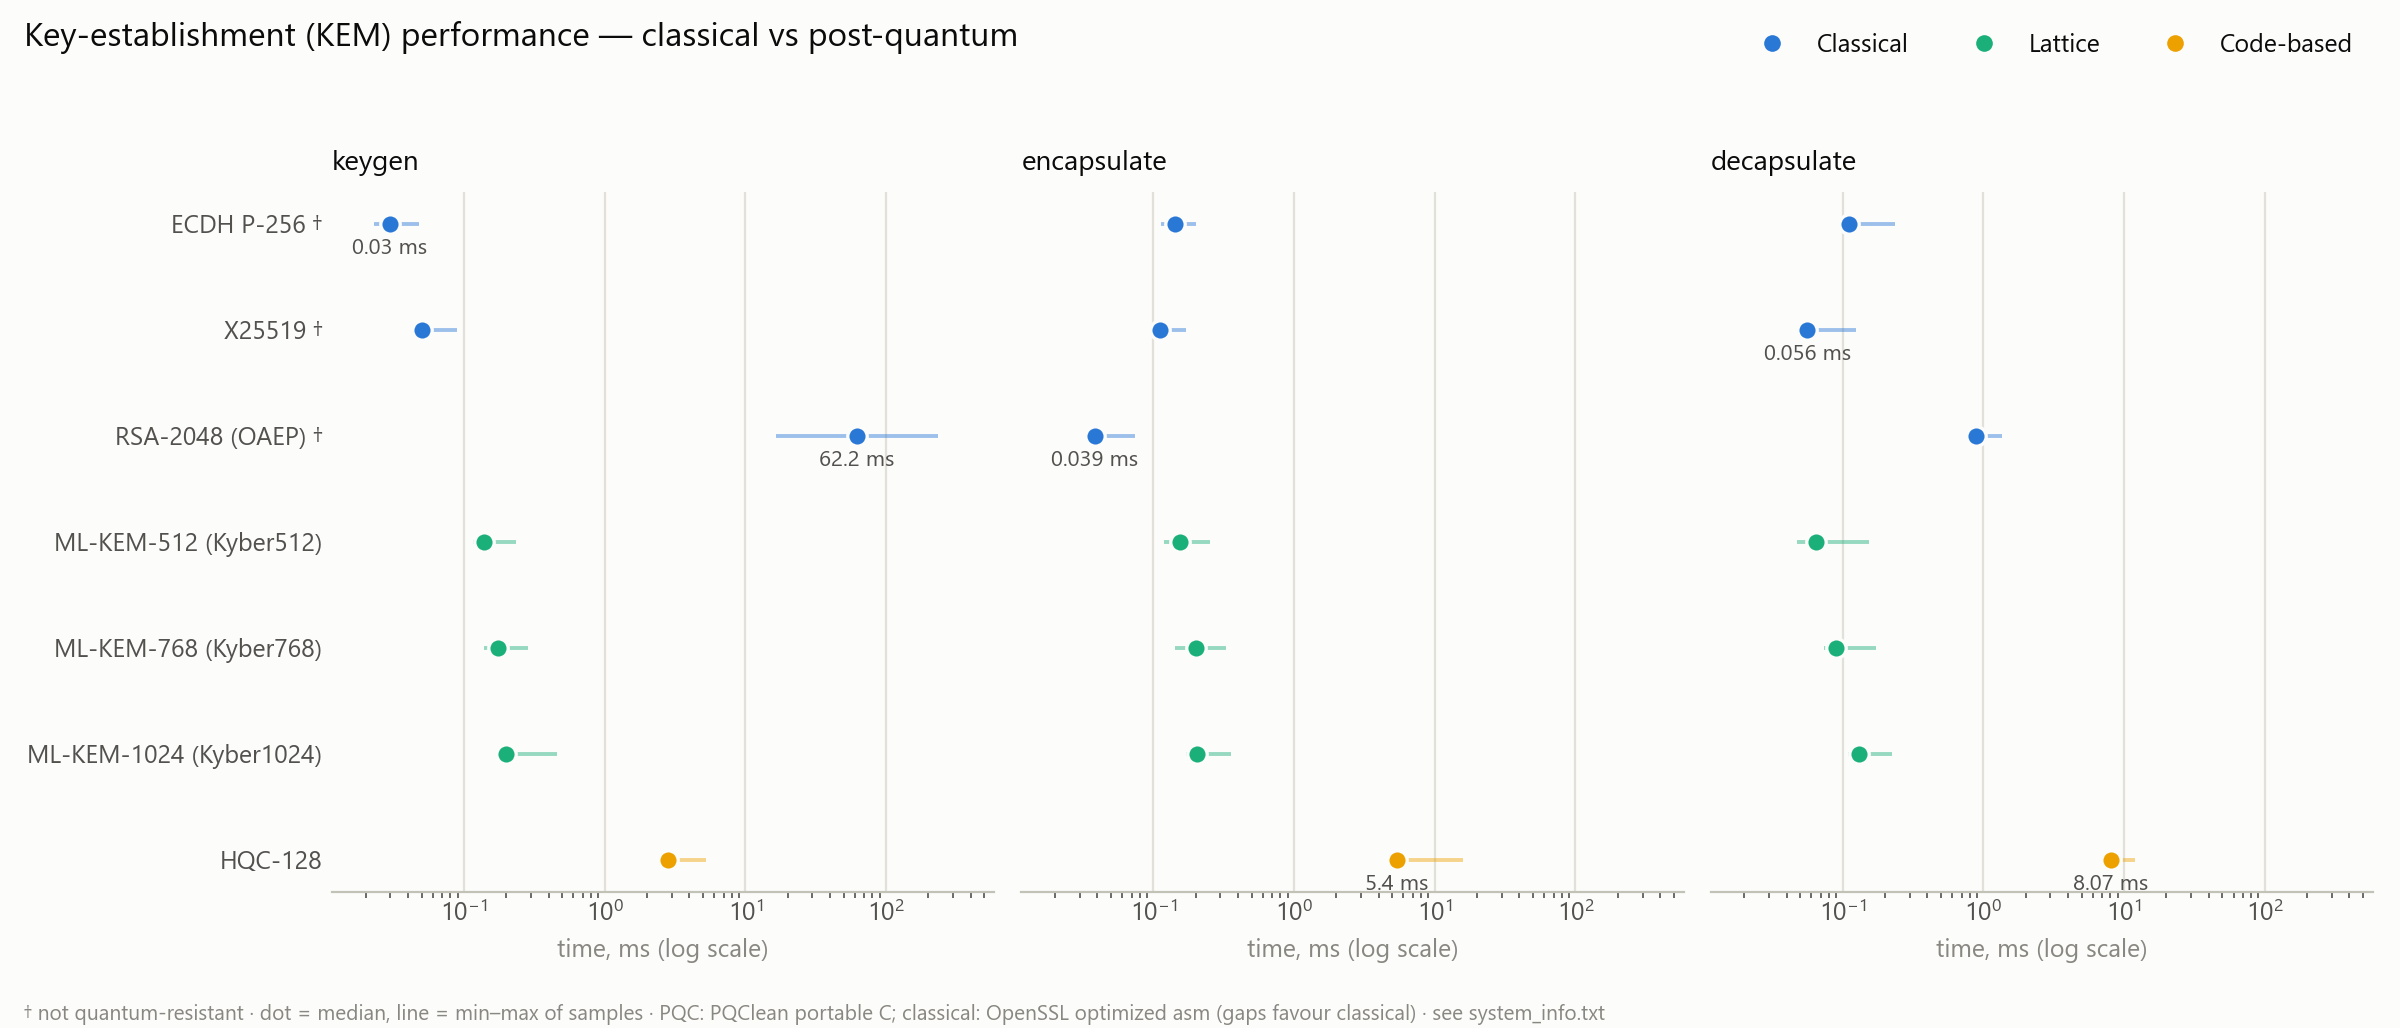
\includegraphics[width=\columnwidth]{fig1_kem_timings.png}
\caption{KEM performance, classical vs.\ post-quantum (log scale).}
\label{fig:kem}
\end{figure}

\begin{figure}[t]
\centering
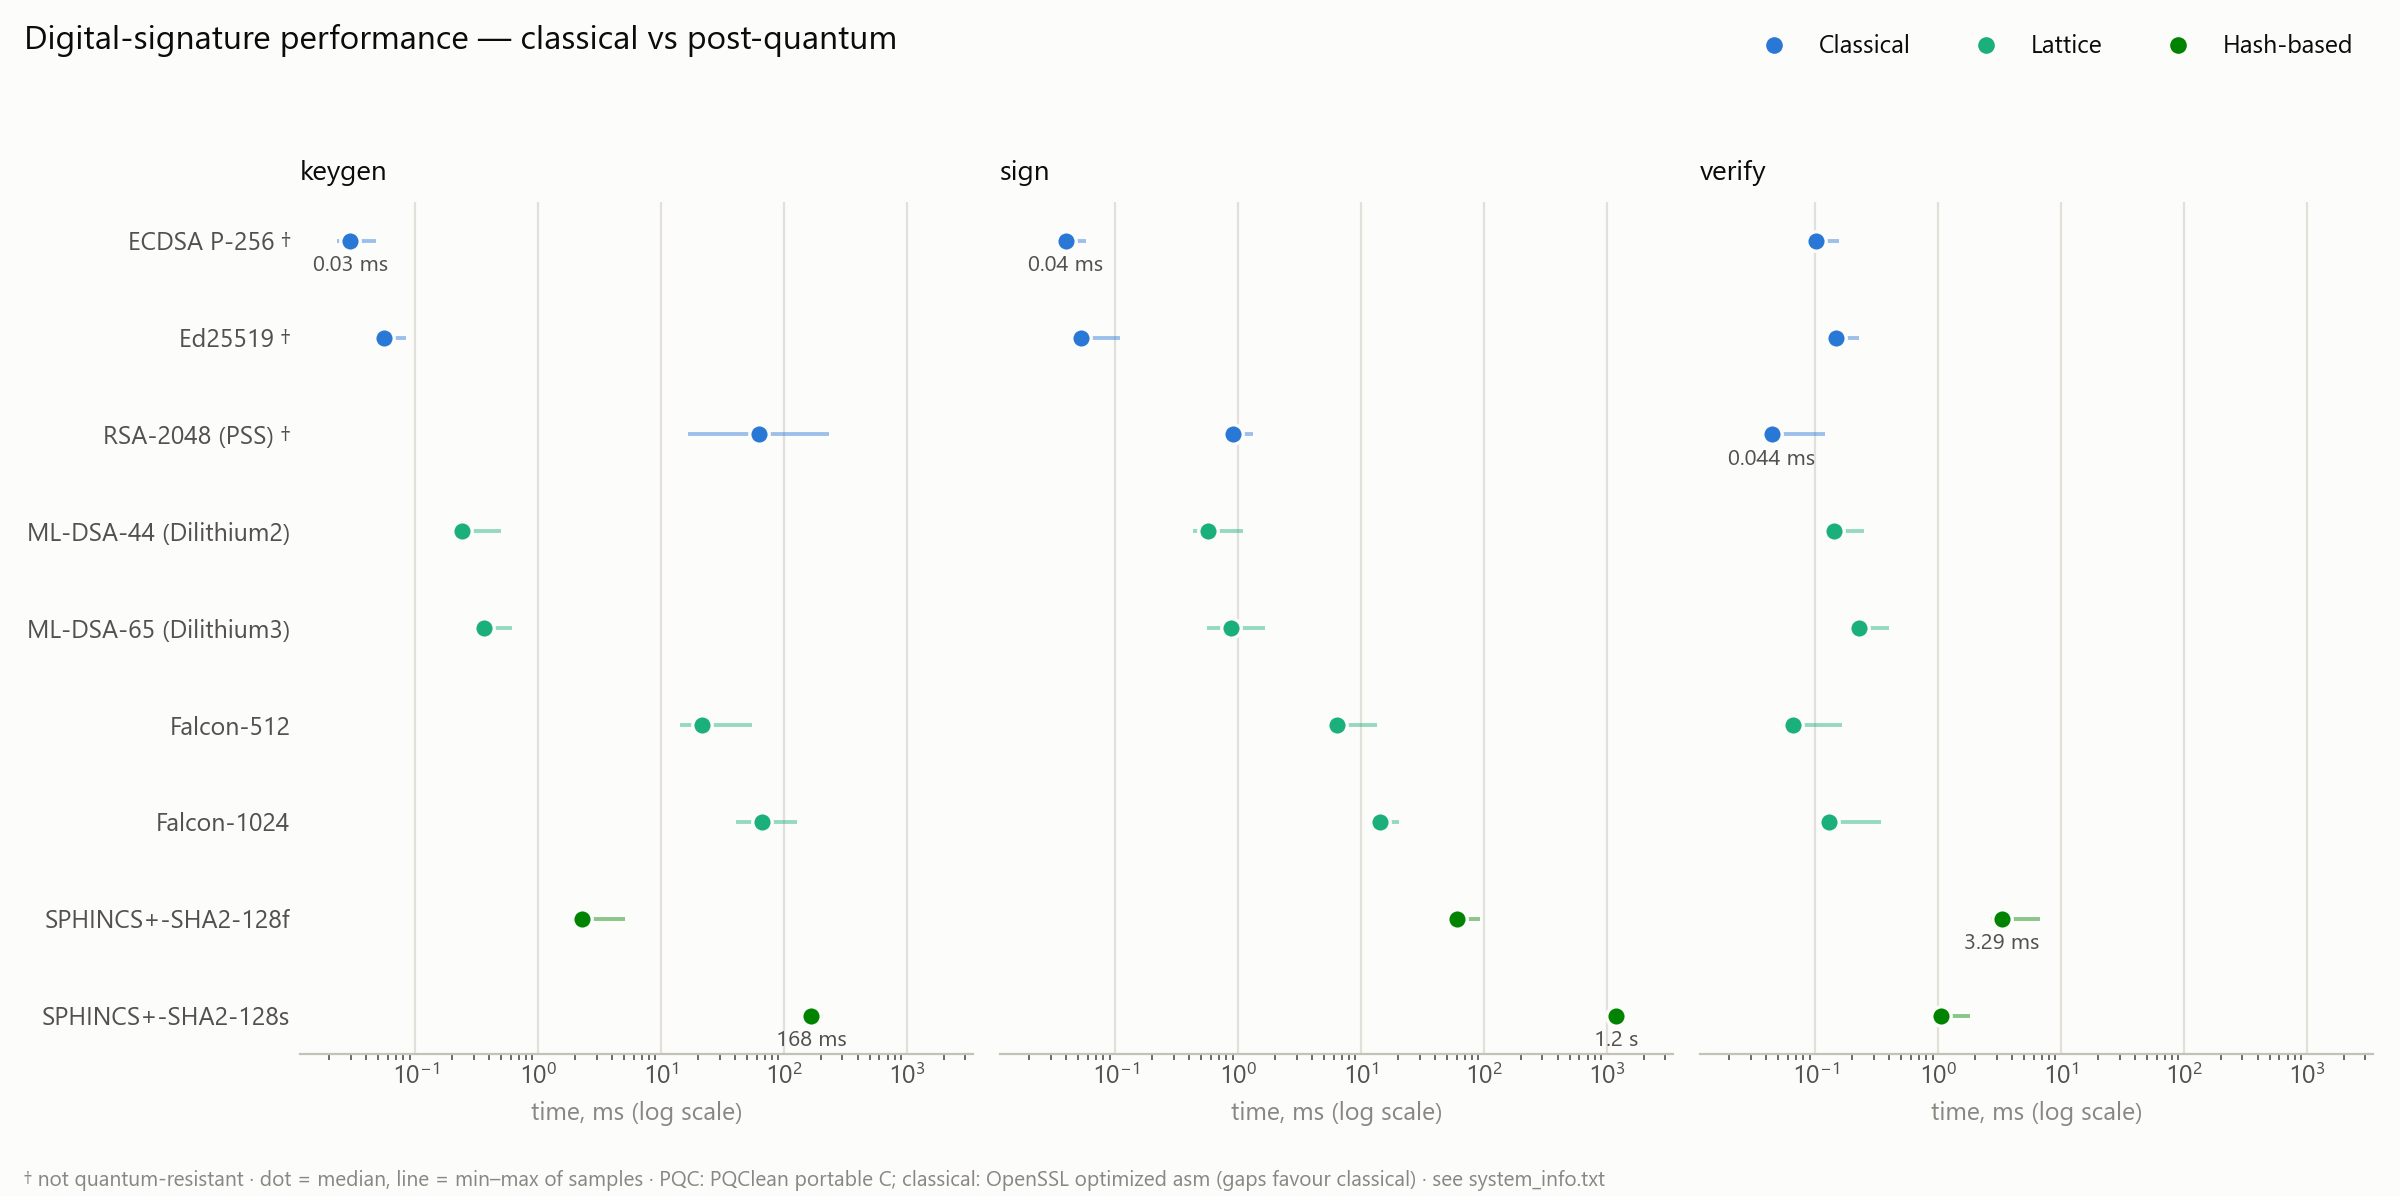
\includegraphics[width=\columnwidth]{fig2_sig_timings.png}
\caption{Signature performance by operation (log scale). Note the
role-dependent asymmetry: Falcon signs slowly but verifies fastest, while
SPHINCS+ signing is three orders of magnitude slower than lattice signing.}
\label{fig:sig}
\end{figure}

\begin{figure}[t]
\centering
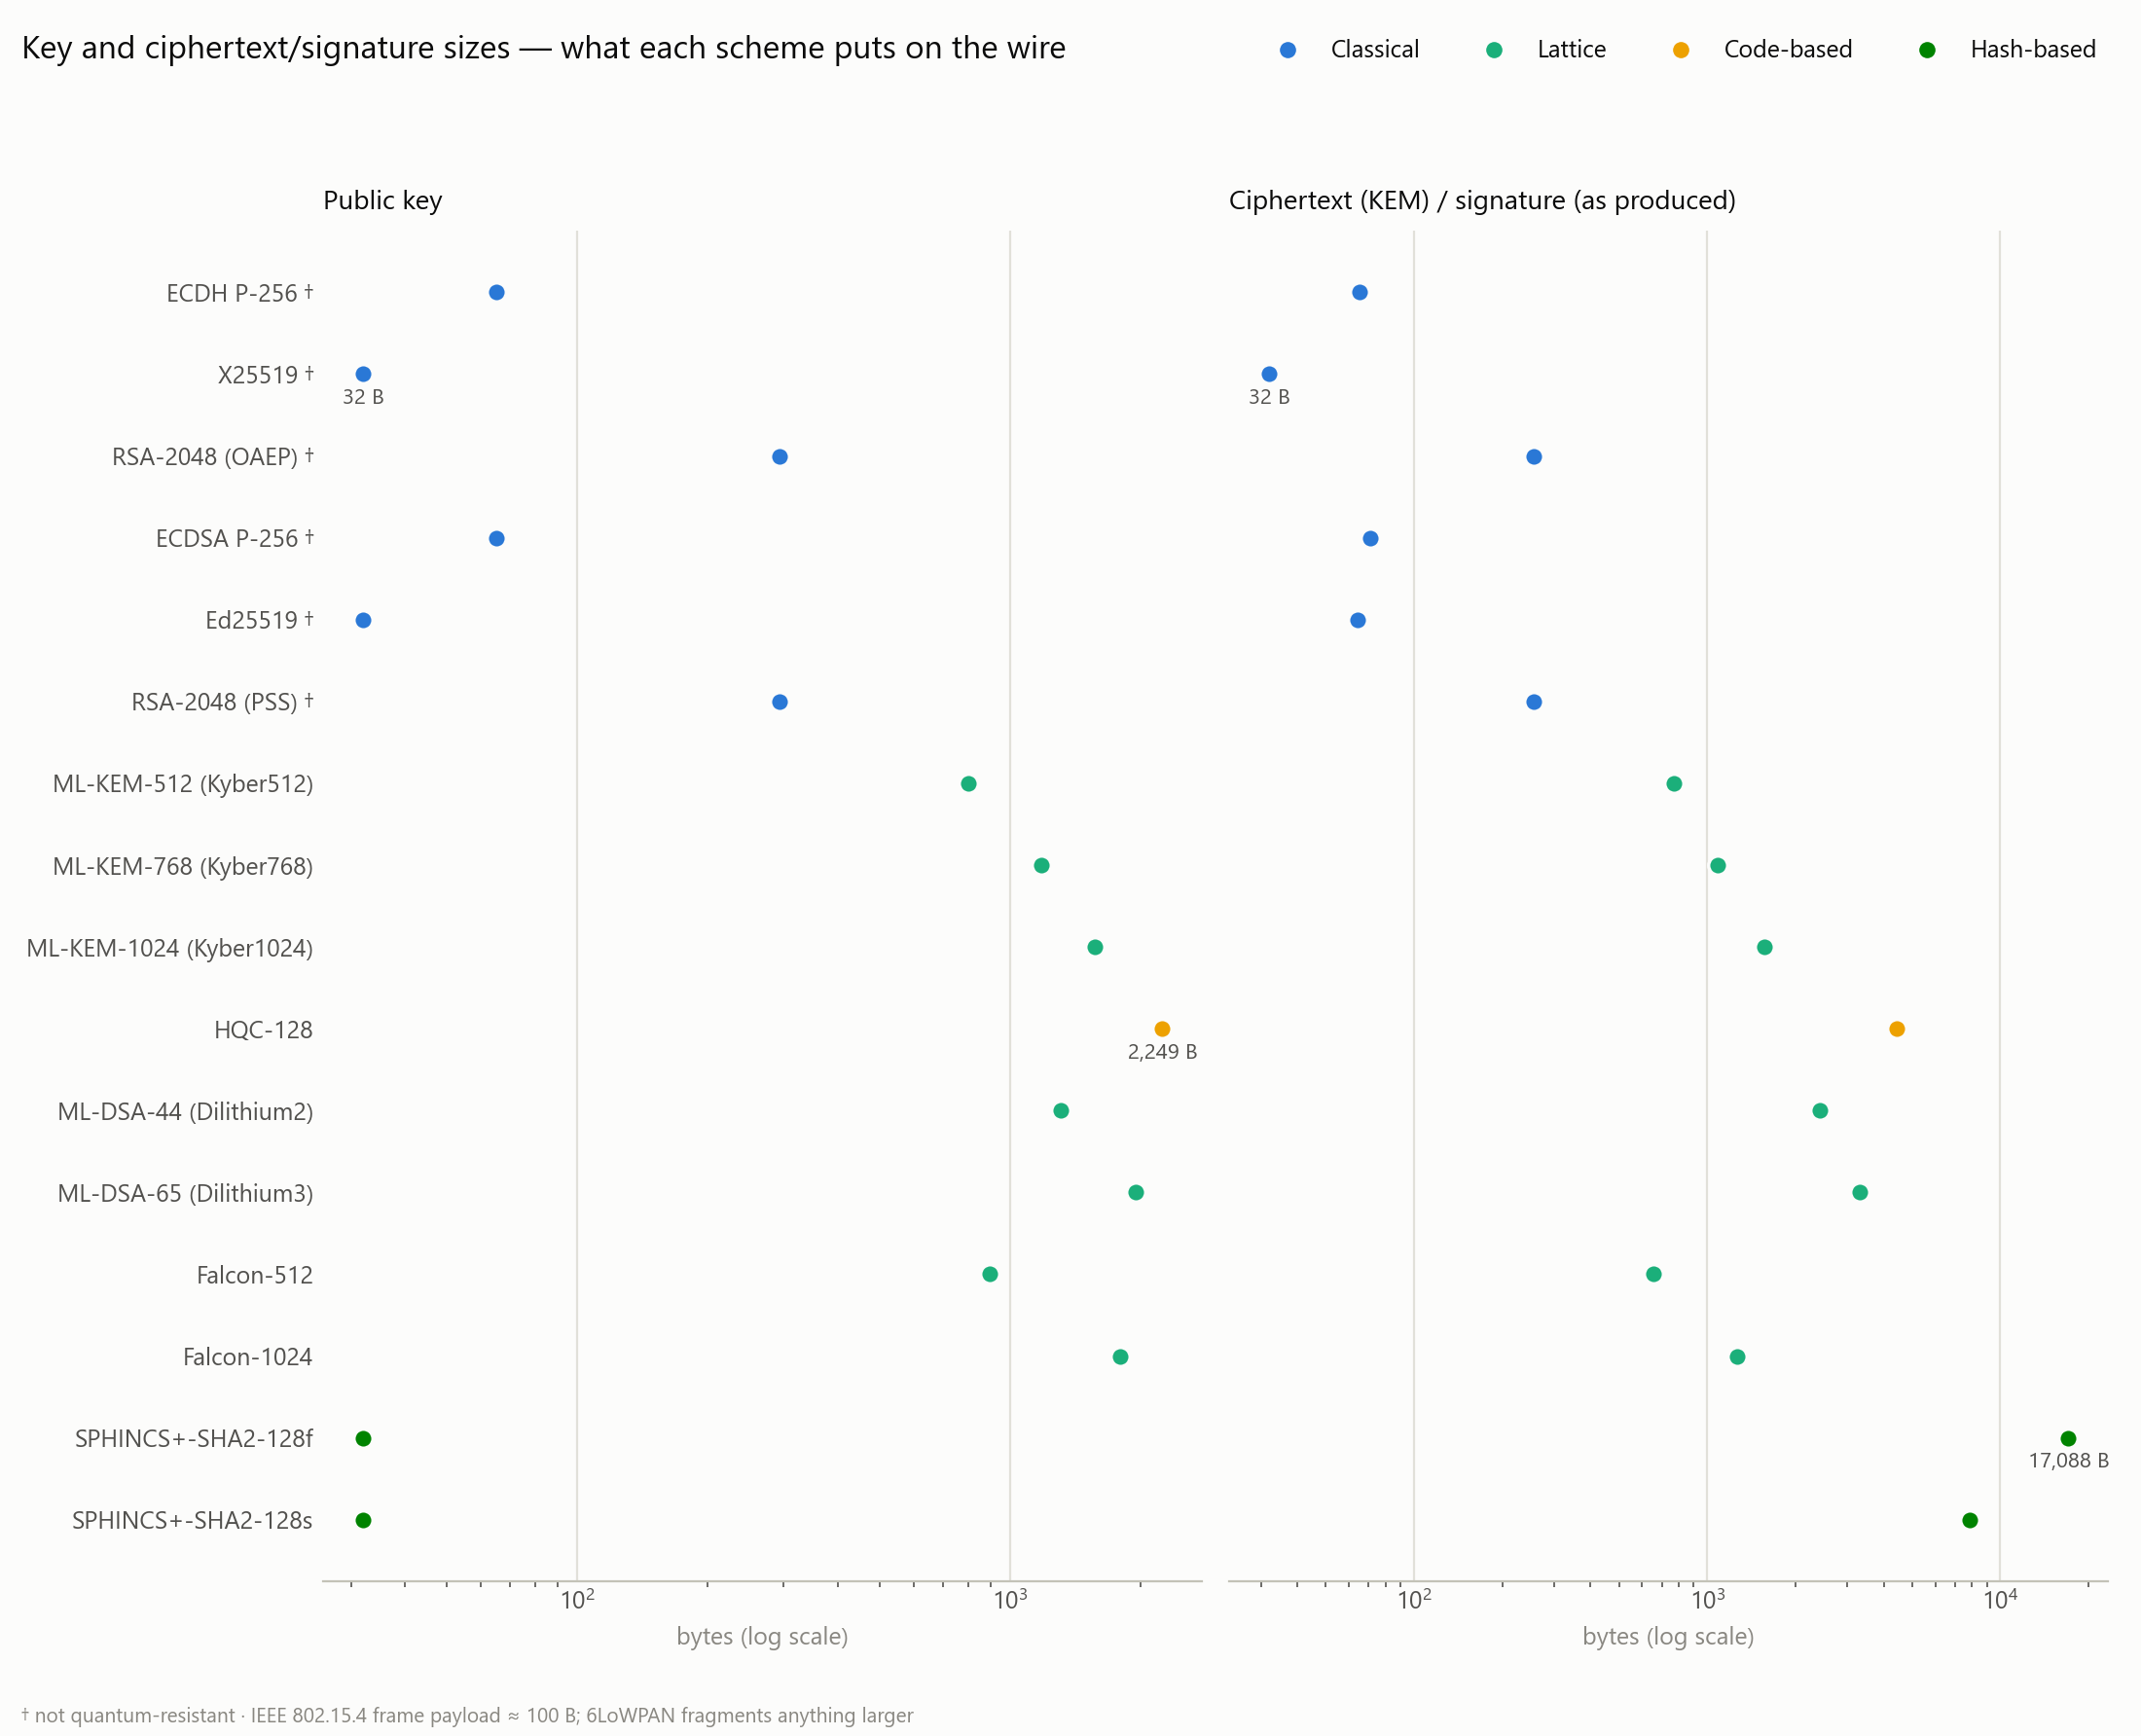
\includegraphics[width=\columnwidth]{fig3_sizes.png}
\caption{Key and ciphertext/signature sizes---the dominant post-quantum cost.
An IEEE~802.15.4 frame carries $\sim$100\,B of payload, so every scheme above
that line fragments.}
\label{fig:sizes}
\end{figure}

\begin{figure}[t]
\centering
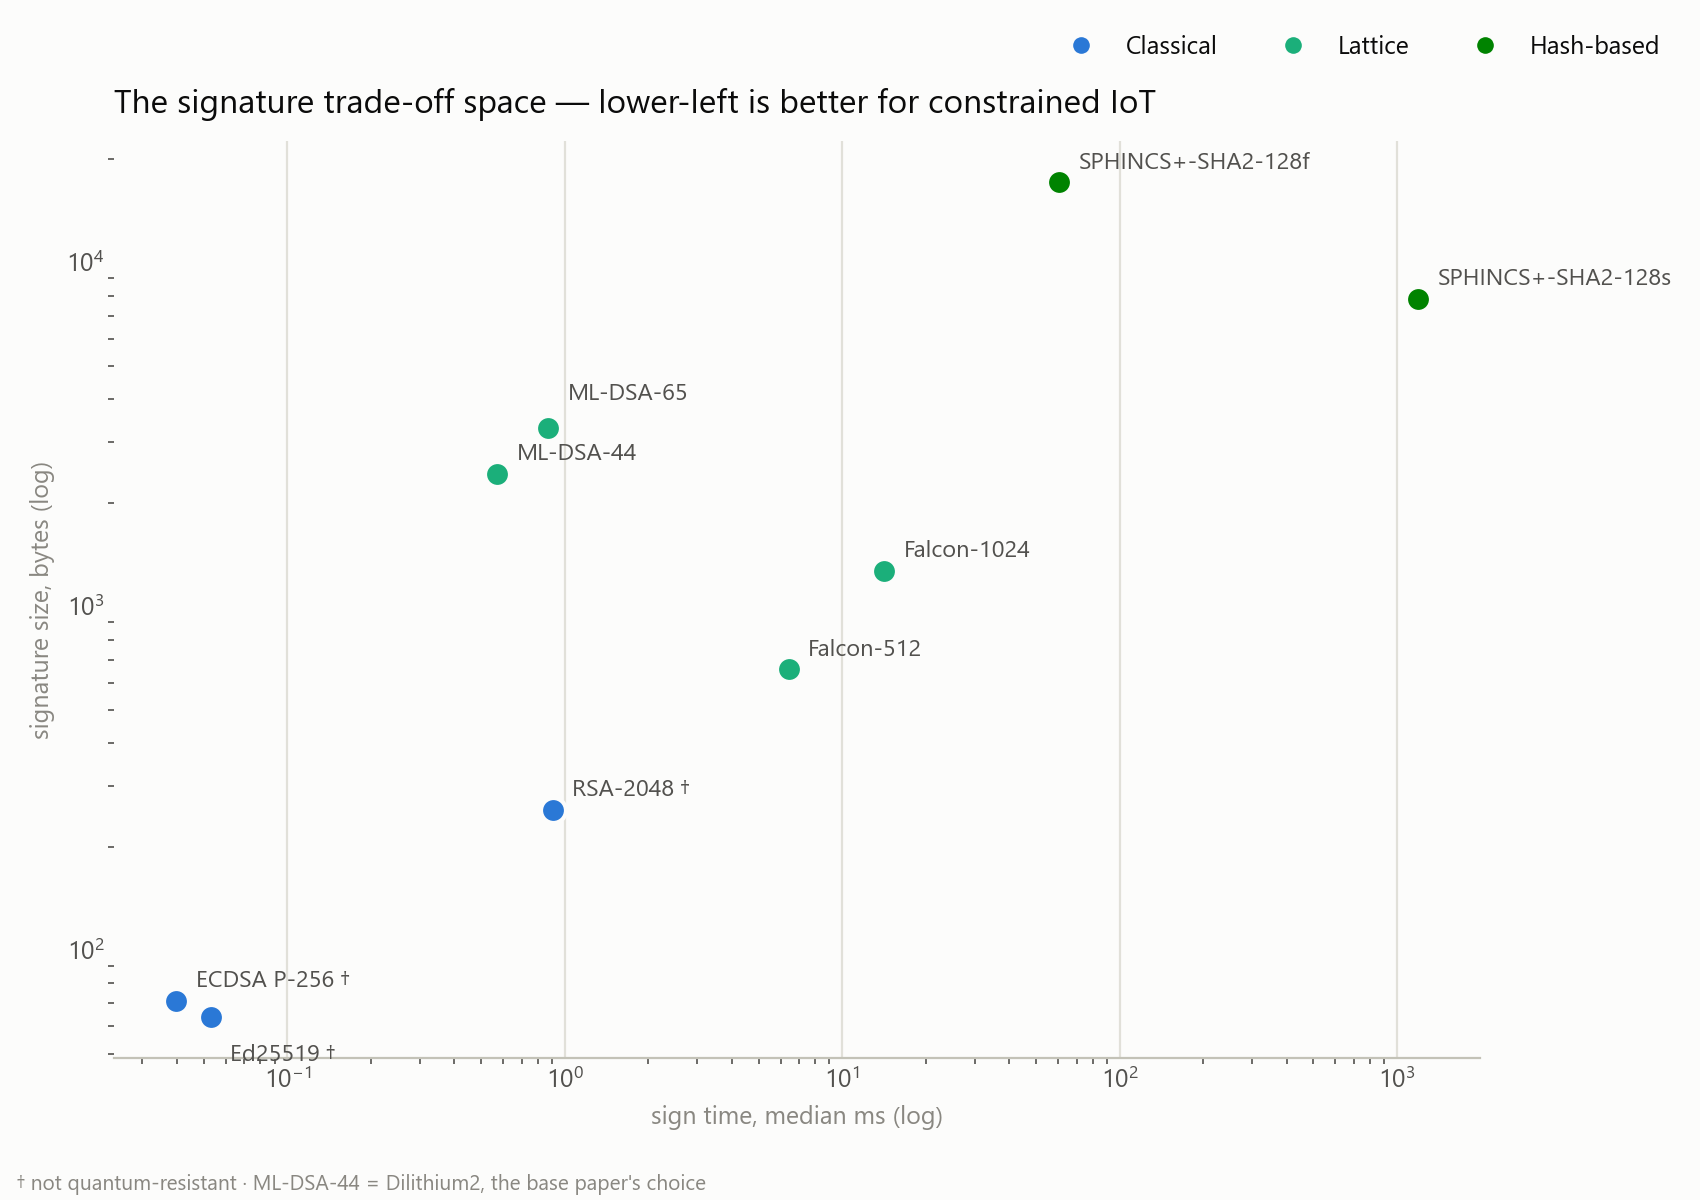
\includegraphics[width=\columnwidth]{fig4_sign_tradeoff.png}
\caption{Signature trade-off space: sign time vs.\ signature size (log-log).
Lower-left is better for constrained IoT.}
\label{fig:tradeoff}
\end{figure}

\textbf{Hybrid key exchange (Gap 1).} Table~\ref{tab:handshake} and
Fig.~\ref{fig:handshake} show the hybrid X25519+ML-KEM-768 handshake (the TLS
1.3 construction) costs only $+64$\,B and $\sim$0.6\,ms over pure ML-KEM-768,
while post-quantum protection over pure classical costs $\sim$2.2\,KB on the
wire. Defence-in-depth against a lattice break is therefore nearly free,
undercutting the base paper's pure-PQC choice.

\begin{table}[t]
\caption{Handshake latency and bytes-on-wire (localhost, 100 runs).}
\label{tab:handshake}
\centering
\small
\begin{tabular}{lrr}
\toprule
Mode & Median (ms) & Total bytes \\
\midrule
classical (X25519) & 1.056 & 202 \\
pure ML-KEM-512 & 1.394 & 1706 \\
pure ML-KEM-768 & 1.642 & 2410 \\
hybrid-512 & 2.076 & 1770 \\
hybrid-768 (TLS X25519MLKEM768) & 2.256 & 2474 \\
\bottomrule
\end{tabular}
\end{table}

\begin{figure}[t]
\centering
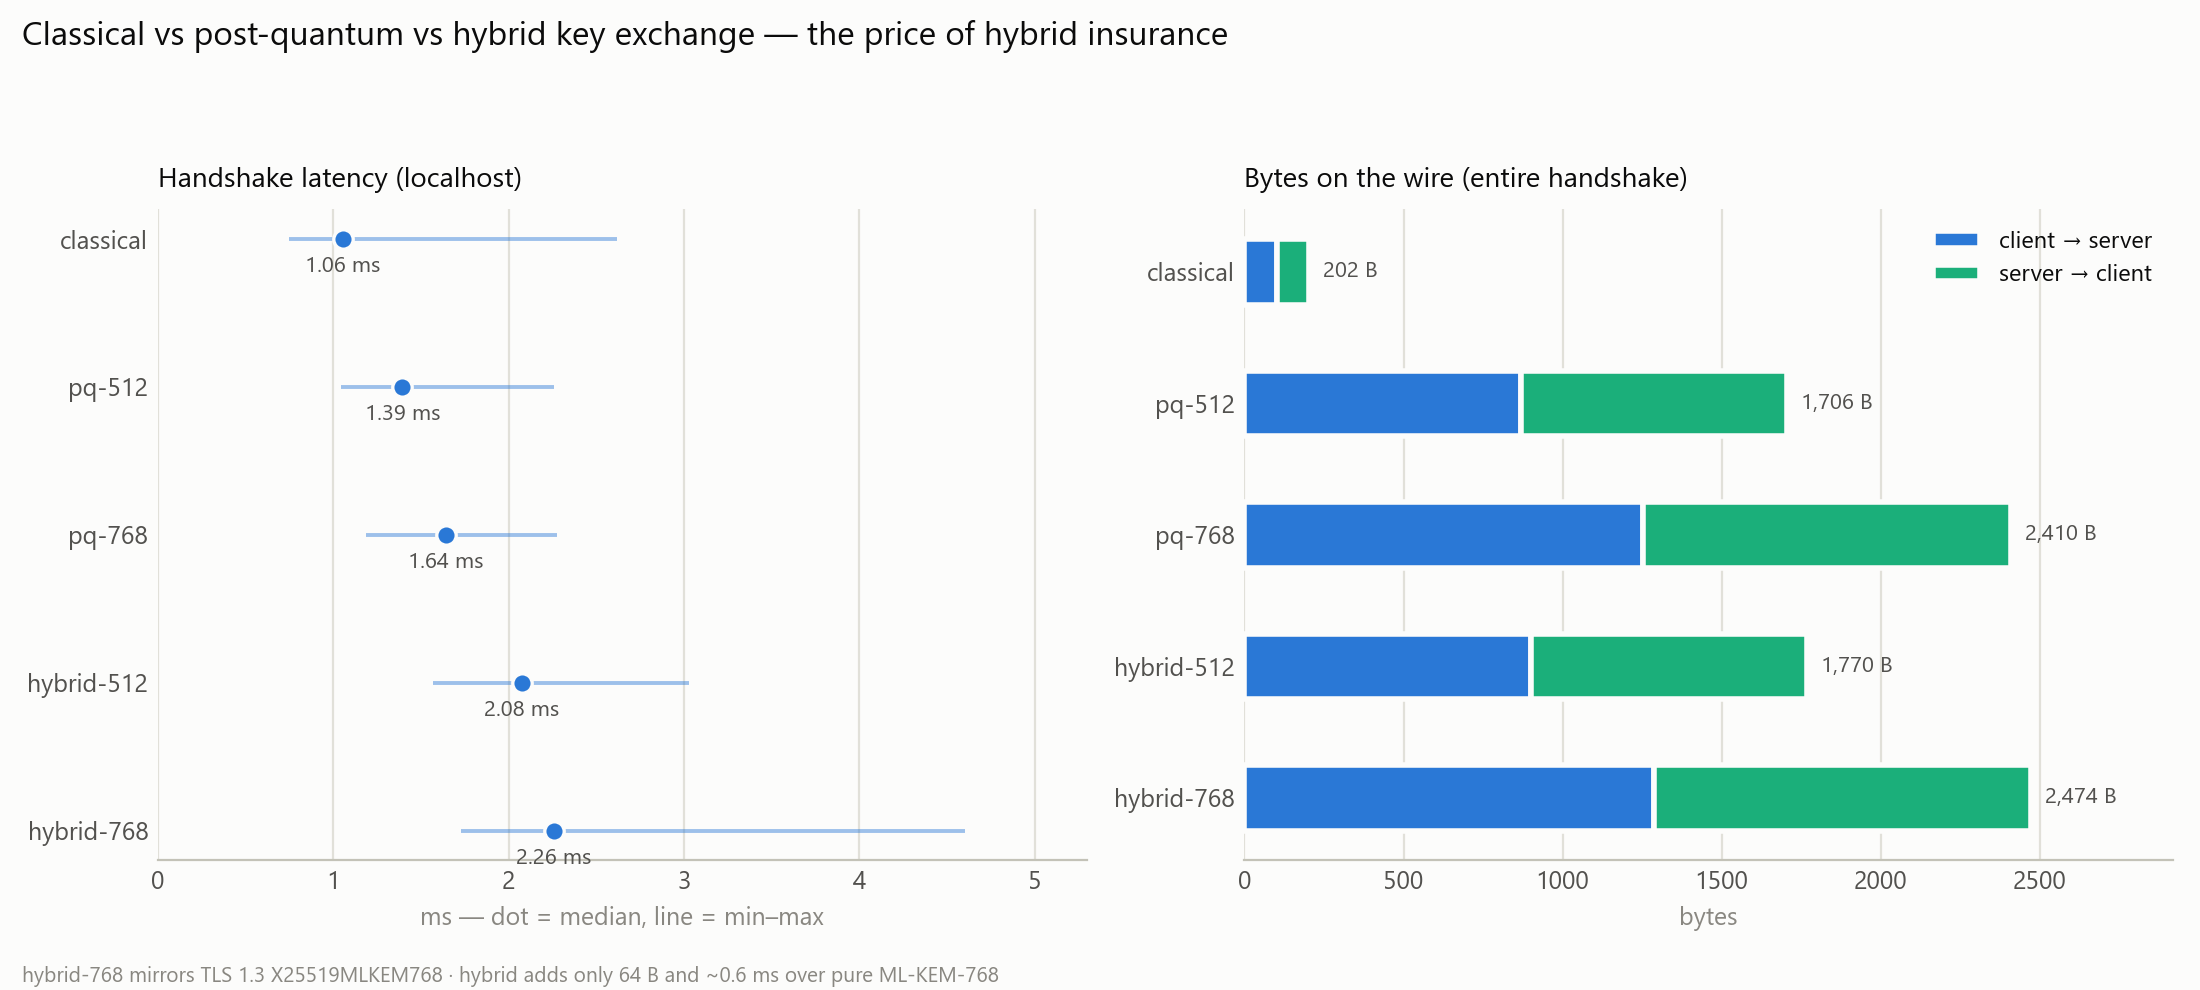
\includegraphics[width=\columnwidth]{fig5_handshake.png}
\caption{Classical vs.\ post-quantum vs.\ hybrid key exchange.}
\label{fig:handshake}
\end{figure}

\textbf{Timing analysis (Gap 4).} Fig.~\ref{fig:timing} shows the naive
early-exit tag comparison leaks perfectly (rejection time rises linearly with
matching prefix, Pearson $r=+1.000$), enabling byte-by-byte tag recovery;
\texttt{hmac.compare\_digest} is flat ($\Delta=0.9$\,ns across the full prefix
range; $z=1.1$, not significant). ML-KEM-512 decapsulation shows no
significant timing difference between valid and corrupted ciphertexts
($|z|\le1.5$, differences $\le$0.03\%): the implicit-rejection path is
constant-time at desktop resolution. Our interleaved design is essential to
this conclusion: a non-interleaved control (regenerable via
\texttt{--sequential}, \texttt{results/timing\_analysis\_sequential.csv})
manufactures a spurious ``oracle risk'' verdict---in the current control run a
$+0.18\%$ phantom difference reported significant at $z\!=\!4.7$, and in an
earlier recorded control as extreme as $z\!=\!-18.9$---caused purely by CPU
state drift over the run, which interleaving eliminates. A naive measurement
design invents a leak that is not there, and more samples would only estimate
the biased value more precisely.

\begin{figure}[t]
\centering
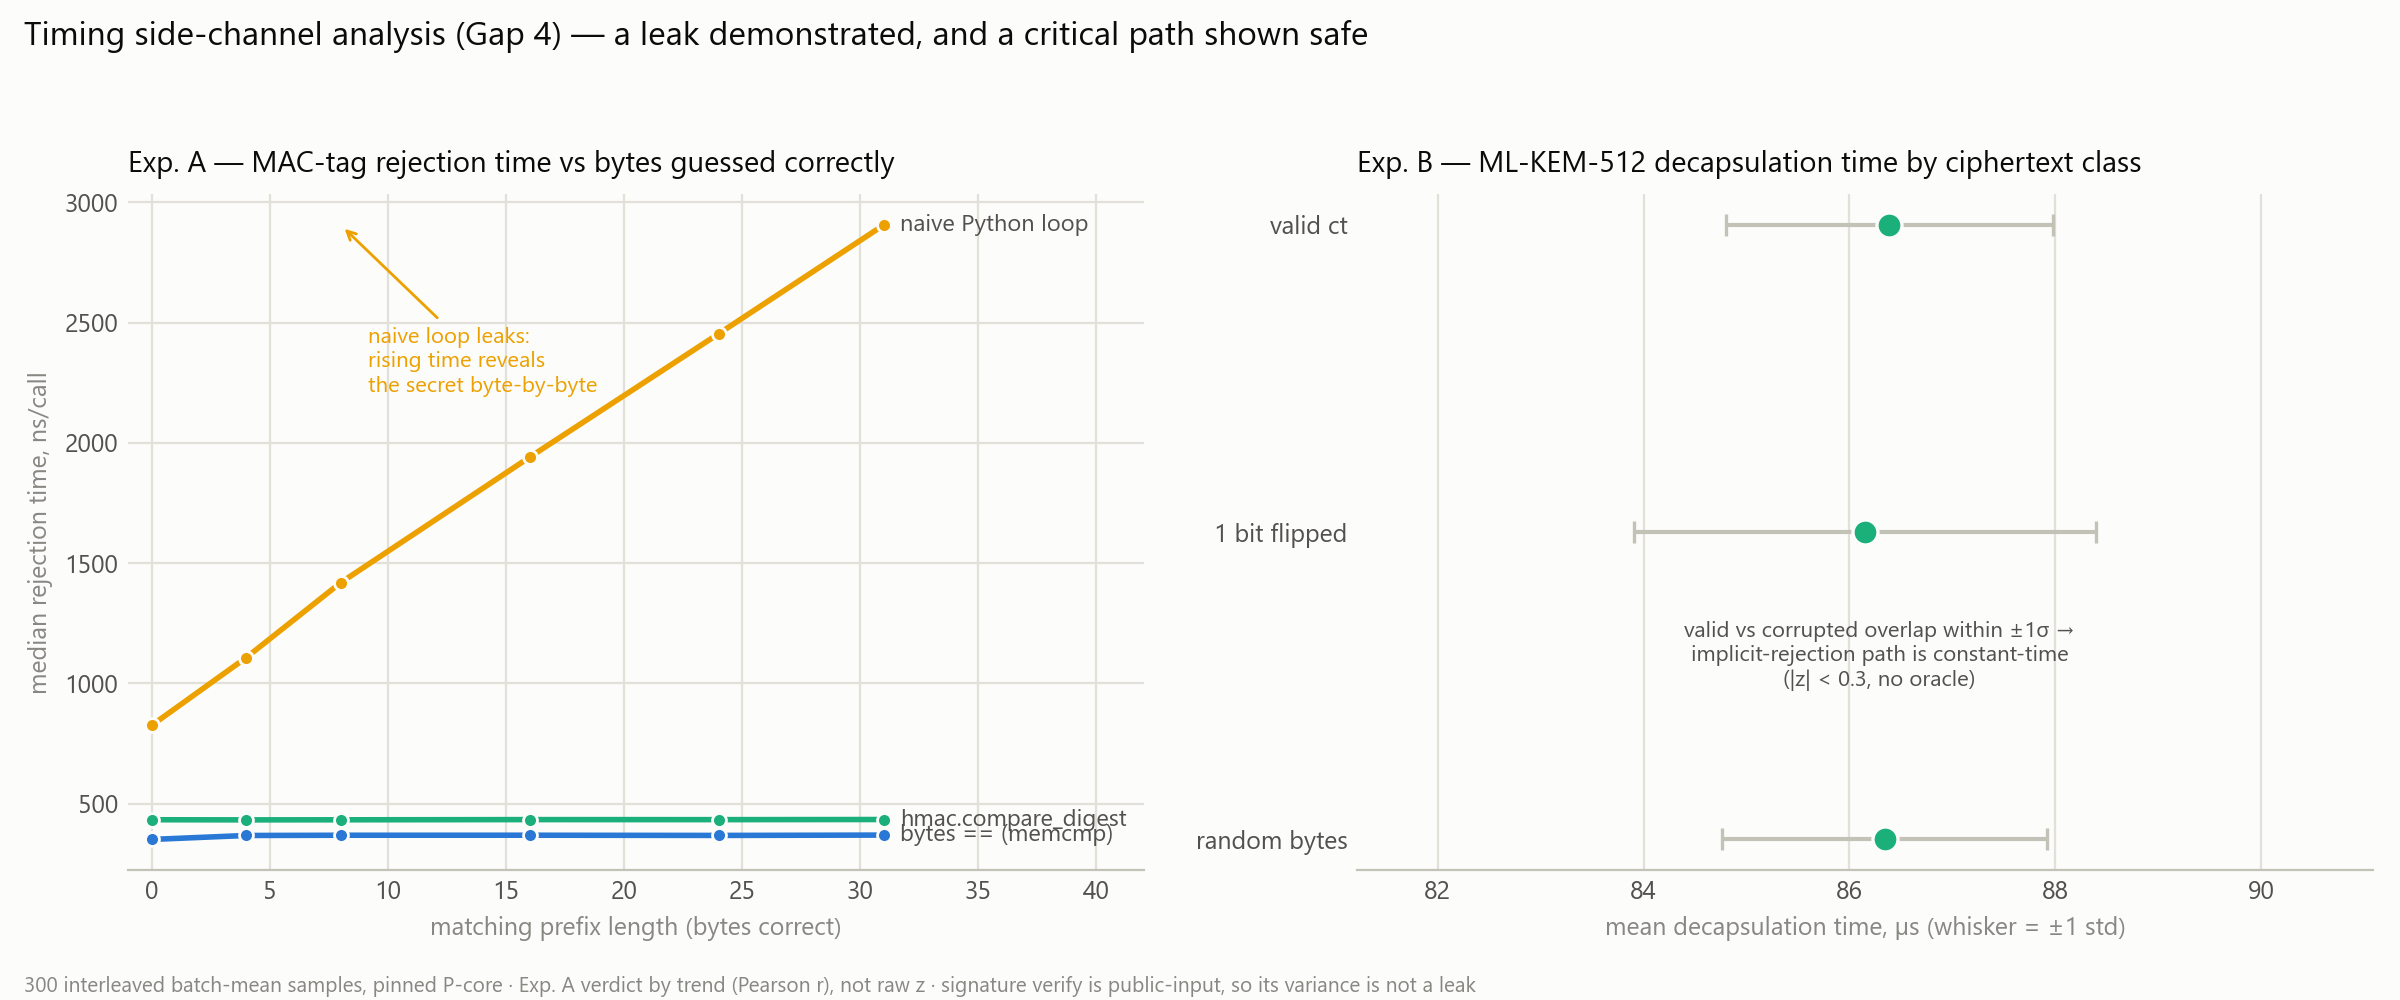
\includegraphics[width=\columnwidth]{fig6_timing.png}
\caption{Timing side-channel analysis: a tag-comparison leak demonstrated
(left) and ML-KEM decapsulation shown constant-time (right).}
\label{fig:timing}
\end{figure}

\textbf{Cortex-M4 extrapolation and the reality check (Gap 5).}
A na\"ive comparison of the paper's latencies against pqm4 milliseconds would be
a clock-mismatch error: pqm4 reports at 24\,MHz by convention, whereas the paper
declares a 120\,MHz device. We therefore apply a \emph{clock-independent} test
(Table~\ref{tab:pqm4}): divide pqm4's measured cycle count by the paper's
reported time to obtain the clock each entry would need in order to be a genuine
cycle-accurate measurement. The four entries imply clocks of 25.0, 28.7, 188.7
and 57.3\,MHz---a 7.5$\times$ spread on one declared device. No processor runs at
four frequencies simultaneously, so these figures cannot all be cycle-accurate
measurements, \emph{whatever} clock is assumed. Normalised instead to the paper's
own 120\,MHz, it is pessimistic on three operations (4.8$\times$, 4.2$\times$,
2.1$\times$) and optimistic on one (0.64$\times$, Dilithium2 signing)---again not
reconcilable by any single scaling. Notably, signing is both the outlier in
direction and the one operation whose cost is data-dependent (Fiat--Shamir with
aborts), which a fixed-cost timing model would under-count; we offer that as a
hypothesis, not a conclusion. This is the core evidence for reporting a
measurement methodology rather than bare numbers.

\begin{table}[t]
\caption{Clock-independent check: the clock each of the paper's reported
latencies would require to be a cycle-accurate measurement, against pqm4's
measured Cortex-M4 cycle counts.}
\label{tab:pqm4}
\centering
\small
\begin{tabular}{llrrr}
\toprule
Scheme & Op & pqm4 cycles & Paper (ms) & Implied clock \\
\midrule
Kyber512 & encaps & 700{,}605 & 28 & 25.0\,MHz \\
Kyber512 & decaps & 888{,}653 & 31 & 28.7\,MHz \\
Dilithium2 & sign & 7{,}925{,}955 & 42 & \textbf{188.7\,MHz} \\
Dilithium2 & verify & 2{,}063{,}096 & 36 & 57.3\,MHz \\
\midrule
\multicolumn{4}{l}{\emph{Declared device clock (paper, Table 3)}} & 120\,MHz \\
\bottomrule
\end{tabular}
\end{table}

\begin{figure}[t]
\centering
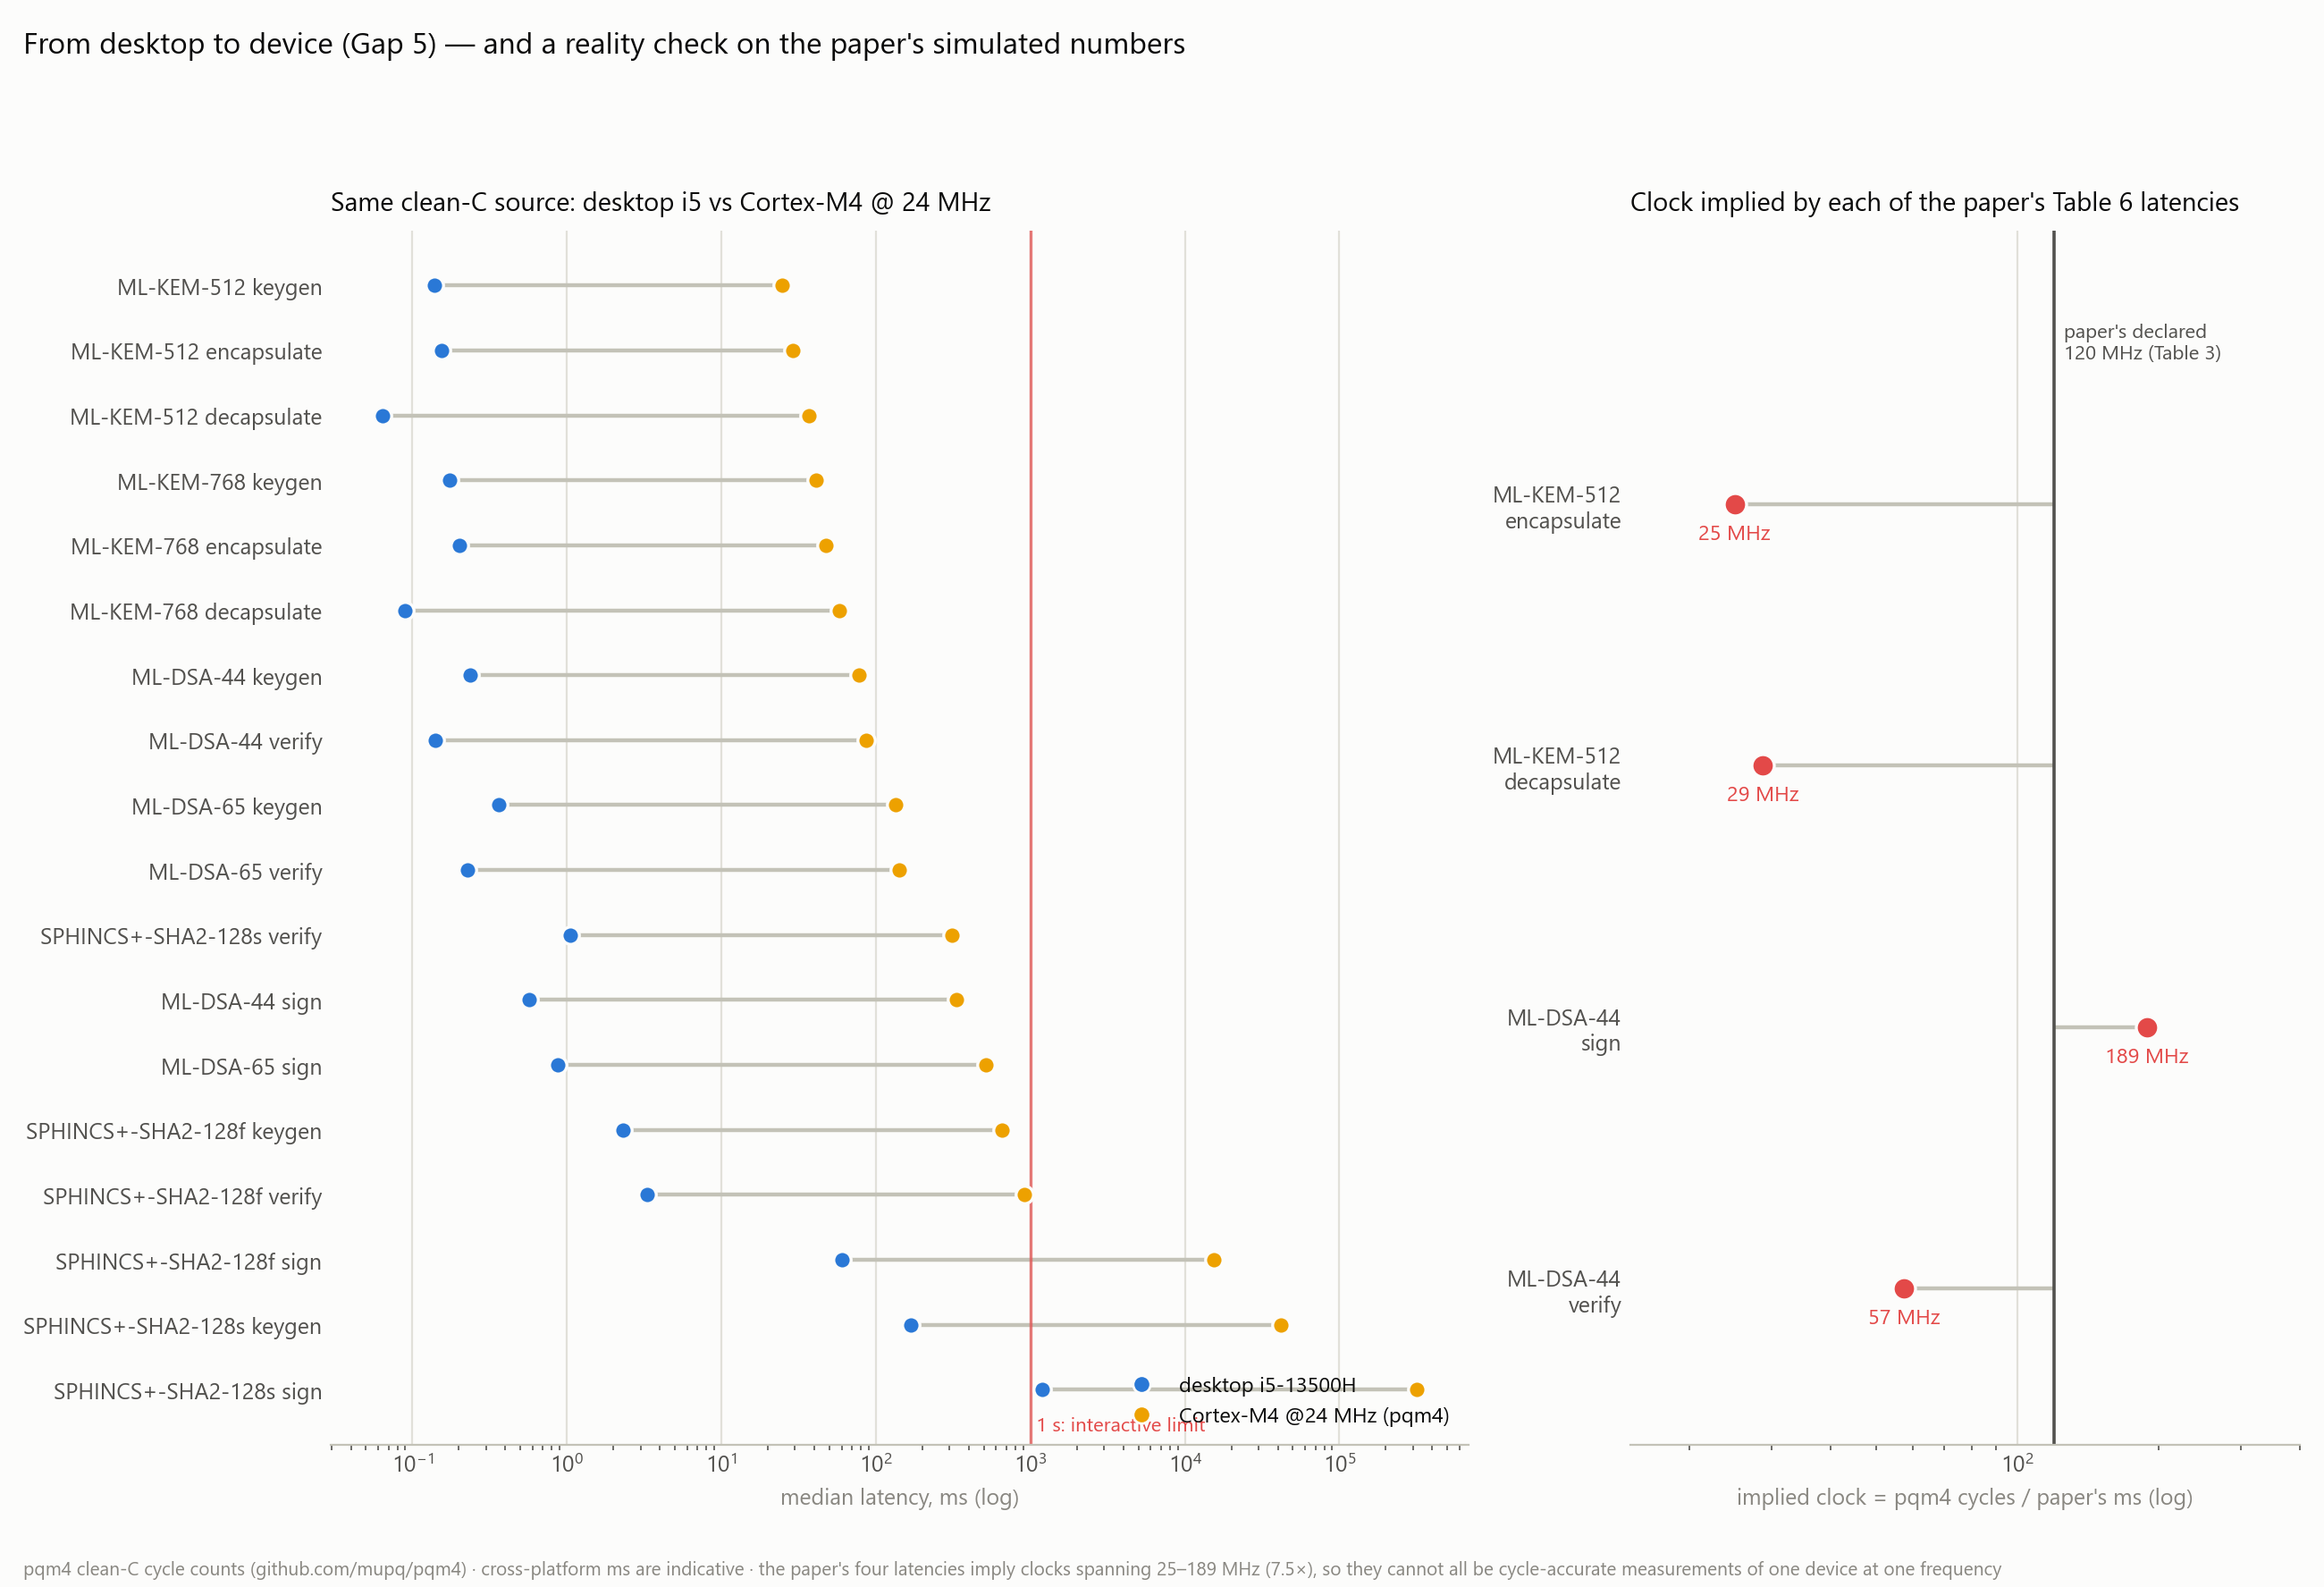
\includegraphics[width=\columnwidth]{fig7_pqm4.png}
\caption{Desktop-to-device gap (left) and the simulated-vs-measured reality
check (right).}
\label{fig:pqm4}
\end{figure}

\textbf{Device-class matrix (Gap 5).} From latency, stack, and size we
recommend: ML-KEM everywhere it fits (the practical floor); ML-DSA for signing
on RFC~7228 Class~2+ (its $\sim$50\,KB signing stack rules out Class~1); Falcon
for \emph{verify-heavy} roles such as firmware-update checking (11\,ms verify,
$\sim$655\,B signature) with keygen/signing offloaded; SPHINCS+ only where signing is
rare and off-device; hybrids wherever the budget allows. Full matrix in
\texttt{results/device\_class\_matrix.csv}.

\section{Discussion and Limitations}
\label{sec:discussion}
Our central reframing: PQShield-IoT treats PQC \emph{computation} as the scarce
resource, but on CPU-class hardware the scarce resource is \emph{bandwidth}
(key/signature sizes), while on Cortex-M4-class hardware computation re-emerges
only for signing-heavy schemes (Dilithium, SPHINCS+), not for ML-KEM. The
correct engineering response is therefore device-class-dependent scheme
selection, which the matrix encodes.

\textbf{Limitations, stated plainly.} (i) The classical baseline is optimised
OpenSSL assembly and PQC is portable C, so classical-vs-PQC gaps are upper
bounds on PQC cost; relative orderings hold only within each implementation
family. (ii) Desktop wall-clock timing on a consumer laptop has tens-of-percent
variance despite core pinning; we report medians and record the environment.
(iii) Cross-platform millisecond comparisons (desktop vs.\ M4) are indicative;
cycle counts are the exact metric. (iv) The timing analysis is black-box and
detects only leaks large relative to the desktop timing noise (Experiment~A's
hundreds-of-nanoseconds tag leak); it cannot resolve few-cycle effects such as
KyberSlash's secret-dependent division, for which instruction-level tools
(\texttt{dudect}) are required. We do not claim to reproduce KyberSlash-scale
sensitivity. (v) We do not
implement authentication in the handshake---it is an ephemeral, unauthenticated
key exchange demonstrating establishment, not a full AKE; authentication is the
role of the signature layer and the base paper's blockchain identities.

\textbf{A forward-secrecy discrepancy.} The base paper claims its primitives
``achieve forward secrecy'' (\S4.9), but its protocol states that every device
holds a \emph{pre-computed} post-quantum key pair and encapsulates against that
long-term $pk_{kem}$ (\S3.2); no ephemeral KEM keypair appears anywhere. Forward
secrecy requires ephemeral keys: with a static key, compromise of $sk_{kem}$
retrospectively recovers the shared secret of every recorded session, and the
paper's KDF does not help because its other inputs (identities, timestamps) are
public. This is precisely the harvest-now-decrypt-later exposure that motivates
post-quantum migration. Our Phase-3 handshake uses ephemeral keys on both legs
and therefore does provide forward secrecy---a concrete demonstration of the
difference.

\textbf{Other observations on the base paper.} We note for
completeness that the base paper describes its ledger inconsistently
(Hyperledger Fabric in Table~3, a Sawtooth validator in \S3.6, a DAG-based
ledger in the same section) and reports differing node counts (15 in \S3.6;
50--200 elsewhere). These are raised as limitations warranting scrutiny, not
as accusations, and lie outside this project's cryptographic scope.

\section{Conclusion and Future Work}
Replacing simulation with measurement wherever a laptop allows, we show that
standardised lattice PQC is computationally cheap on CPU-class devices (its
cost is bandwidth), that hybrid key exchange is nearly free insurance, that a
representative decapsulation path is constant-time while a naive tag comparison
is not, and that the base paper's four reported cryptographic latencies imply
mutually incompatible processor clocks (25--189\,MHz) when checked against
measured Cortex-M4 cycle counts. Future work:
authenticated hybrid handshakes with PQ signatures; on-hardware measurement on
a Cortex-M4 board; instruction-level constant-time verification; and integrating
the device-class matrix into an adaptive scheme-selection layer.

\bibliographystyle{IEEEtran}
\bibliography{references}

\end{document}
